\documentclass[conference]{IEEEtran}
\IEEEoverridecommandlockouts
\usepackage{cite}
\usepackage{amsmath,amssymb,amsfonts}
\usepackage{graphicx}
\usepackage{textcomp}
\usepackage{xcolor}
\usepackage{booktabs}
\usepackage{array}
\usepackage[most]{tcolorbox}
\usepackage{tikz}
\usetikzlibrary{arrows.meta,positioning,calc,fit,backgrounds}
\usepackage{url}
\def\UrlBreaks{\do\/\do-\do.\do_}
\usepackage[hidelinks]{hyperref}

\definecolor{navy}{HTML}{1F4E79}
\definecolor{rust}{HTML}{C0504D}
\definecolor{leaf}{HTML}{4F7F3A}
\newtcolorbox{contrib}{colback=navy!4,colframe=navy!70,boxrule=0.6pt,arc=1.5pt,left=3pt,right=3pt,top=2pt,bottom=2pt,
  fonttitle=\bfseries\small,title=Key contributions of this work}
\newcommand{\novel}[1]{\textcolor{navy}{\textbf{#1}}}

\begin{document}

\title{A Single-Package CMOS Heterodyne Theremin with Logic-Gate Mixing and Hybrid Potentiometer--Antenna Pitch Control}

\author{
\IEEEauthorblockN{Chetansai Mihir P}
\IEEEauthorblockA{\textit{Dept. of Electrical and}\\ \textit{Electronics Engineering}\\
\textit{Vellore Institute of Technology}\\
Vellore, India\\
mihirpuramsetti@gmail.com}
\and
\IEEEauthorblockN{Nainika Karthik}
\IEEEauthorblockA{\textit{Dept. of Electrical and}\\ \textit{Electronics Engineering}\\
\textit{Vellore Institute of Technology}\\
Vellore, India\\
nainika.karthik@gmail.com}
\and
\IEEEauthorblockN{P Vigneshvaran}
\IEEEauthorblockA{\textit{Dept. of Electrical and}\\ \textit{Electronics Engineering}\\
\textit{Vellore Institute of Technology}\\
Vellore, India\\
p.vigneshvaran2007@gmail.com}
\and
\IEEEauthorblockN{Rithikhaasree T}
\IEEEauthorblockA{\textit{Dept. of Electrical and}\\ \textit{Electronics Engineering}\\
\textit{Vellore Institute of Technology}\\
Vellore, India\\
rithikhaathegreat@gmail.com}
}

\maketitle

\begin{abstract}
A theremin is played without touch: the player's hand forms a small, distance-dependent capacitance with an antenna, and a heterodyne (beat-frequency) circuit turns that sub-picofarad change into an audible pitch. Classical designs need hand-wound inductors and careful LC tuning. This paper presents an inductor-free theremin in which a \emph{single} CD4093BE quad Schmitt-trigger NAND package performs every radio-frequency function: two matched $\approx$692\,kHz RC oscillators, a logic-gate mixer, and a level-shifting inverter. An MCP602 Sallen--Key filter removes the carrier, and an LM386 drives an 8\,$\Omega$ speaker, all from one 9\,V battery through a 7805 regulator. We derive (i) an oscillator model that includes Schmitt thresholds, propagation delay and the resulting threshold overshoot, which shows that the common $1/(1.2RC)$ rule overestimates the frequency by 20\%; (ii) a closed-form result showing that the filtered output of a logic-gate mixer is a \emph{triangle wave} at the beat frequency with a peak-to-peak amplitude of $V_{DD}D$, which sets the instrument's timbre; and (iii) an antenna sensitivity of 3.9\,kHz/pF. A hybrid potentiometer--antenna control scheme sets the base pitch and keeps the oscillators away from their lock-in region. A full-circuit SPICE simulation agrees with every analytical oscillator value to within 0.05\%, and a breadboard prototype produced a smooth, continuous, contactless pitch response over a 5--25\,cm hand range.
\end{abstract}

\begin{IEEEkeywords}
theremin, heterodyne, beat frequency, CD4093, Schmitt trigger, relaxation oscillator, capacitive sensing, logic-gate mixer, Sallen--Key filter, LM386
\end{IEEEkeywords}

%=====================================================================
\section{Introduction}
The theremin, patented by L.~S.~Theremin in 1928~\cite{theremin1928}, is one of the very few instruments played without touch. The hand and a metal antenna form a capacitor of well under a picofarad to a few picofarads. That is far too small to change the pitch of an audio oscillator audibly, so the instrument runs two radio-frequency (RF) oscillators and listens to their \emph{difference}. A tiny fractional change at RF then becomes a large change in the audible beat note~\cite{skeldon1998}. Vacuum-tube and later transistor designs~\cite{moog1961,glinsky2000} build these oscillators from LC tanks, which require inductors, careful layout and tuning.

This work asks how far the heterodyne theremin can be simplified while keeping solid engineering behind every stage. Starting from a two-IC hobbyist idea that uses CMOS Schmitt-trigger oscillators~\cite{greatscott}, we built a complete speaker-driving instrument with three ICs, no inductors and one 9\,V battery. We also supply the analysis that such minimal designs usually lack.

\begin{contrib}
\small
\begin{enumerate}\setlength{\itemsep}{1pt}
\item \novel{Single-package RF front end.} All four gates of one CD4093BE are used: two oscillators, a mixer and an inverter. Both oscillators share one die and one supply, so their drift is common-mode and largely cancels in the beat note.
\item \novel{Analytic logic-mixer model.} The filtered output of a NAND/AND mixer is shown to be a triangle wave at $|f_A-f_B|$ with amplitude $V_{DD}D$, with harmonics falling as $1/n^2$. The inverter stage is shown to be necessary to keep this signal inside the op-amp's input range.
\item \novel{Hybrid potentiometer--antenna pitch control.} A pitch pot in the antenna oscillator zero-beats the instrument, sets a base note, and keeps the operating point on the side of zero beat where pitch rises monotonically, away from the injection-locking dead zone.
\item \novel{Portable single-supply design, verified in SPICE.} One 9\,V battery and a 7805 power every stage from one 5\,V rail. Every design value is cross-checked against a full-circuit simulation.
\end{enumerate}
\end{contrib}

Section~\ref{sec:bg} reviews theremin topologies, Section~\ref{sec:arch} presents the architecture, and Section~\ref{sec:design} analyses each stage. Sections~\ref{sec:impl} and~\ref{sec:results} cover the implementation and results, and Section~\ref{sec:disc} discusses limitations.

%=====================================================================
\section{Background}\label{sec:bg}
In a heterodyne theremin, a \emph{variable} oscillator at $f_A$ includes the hand capacitance $C_h$, and a \emph{reference} oscillator runs at a fixed $f_B$. A nonlinear mixer produces components at $f_A\pm f_B$, and a low-pass filter keeps only the beat $f_b=|f_A-f_B|$. The benefit is a \emph{relative-sensitivity gain}:
\begin{equation}
\frac{\Delta f_b}{f_b}=\frac{f_A}{f_b}\cdot\frac{\Delta f_A}{f_A}.
\label{eq:gain}
\end{equation}
At $f_A\approx692$\,kHz and $f_b=1$\,kHz, a fractional change of the oscillator becomes a 692$\times$ larger fractional change of pitch. A single audio oscillator could only respond to picofarads if its timing capacitor were itself a few picofarads, which would need gigaohm resistors to reach audio frequencies and is not practical. Table~\ref{tab:compare} compares representative approaches.

\begin{table}[!t]
\centering
\caption{Comparison of theremin topologies}
\label{tab:compare}
\setlength{\tabcolsep}{3pt}
\renewcommand{\arraystretch}{1.1}
\footnotesize
\begin{tabular}{@{}p{1.65cm}p{1.6cm}p{1.45cm}p{0.75cm}p{1.3cm}@{}}
\toprule
Design & Oscillators & Mixer & Induc\-tors & Output \\
\midrule
Theremin~\cite{theremin1928} & Vacuum-tube LC & Vacuum tube & Yes & Speaker \\
Moog~\cite{moog1961} & Transistor LC & Transistor & Yes & Ext.\ amplifier \\
Two-IC idea~\cite{greatscott} & CMOS Schmitt RC & Op-amp & No & Line level \\
\textbf{This work} & \textbf{CMOS Schmitt RC, one package} & \textbf{NAND gate + active filter} & \textbf{No} & \textbf{8\,$\Omega$ speaker, 9\,V battery} \\
\bottomrule
\end{tabular}
\end{table}

%=====================================================================
\section{System Architecture}\label{sec:arch}
Fig.~\ref{fig:block} shows the signal chain and Fig.~\ref{fig:sch} the complete schematic, which is divided into six numbered blocks. Block~1 contains the antenna oscillator U1A, whose timing node is wired to the antenna, and the fixed reference oscillator U1B. In Block~2, gate U1C mixes the two square waves and U1D inverts the result. Block~3 is U2A, one half of the rail-to-rail MCP602, configured as a unity-gain second-order Sallen--Key low-pass filter~\cite{sallenkey1955,franco2015} that removes the carrier. Block~4 contains a fixed attenuator, the volume control and the LM386 amplifier, which drives the speaker. Blocks~5 and~6 hold the supply, the decoupling and the unused op-amp half.

\begin{figure}[!t]
\centering
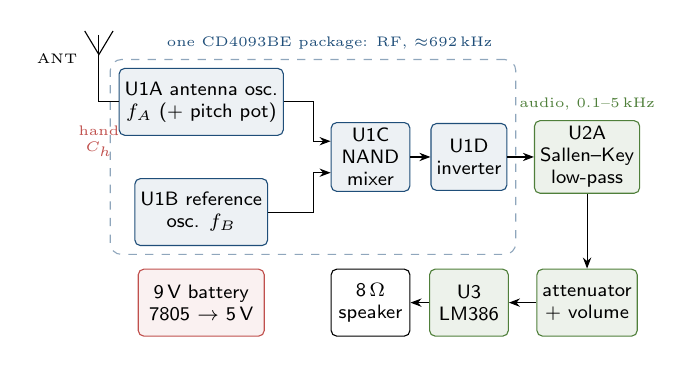
\begin{tikzpicture}[
  font=\scriptsize\sffamily, >={Stealth[length=4pt]},
  blk/.style={draw, rounded corners=2pt, align=center, minimum height=0.85cm, inner sep=2pt, fill=white},
  rf/.style={blk, fill=navy!8, draw=navy},
  au/.style={blk, fill=leaf!10, draw=leaf},
  pw/.style={blk, fill=rust!8, draw=rust}]
\node[rf, minimum width=1.6cm] (A) at (0,0.7) {U1A antenna osc.\\$f_A$ (+ pitch pot)};
\node[rf, minimum width=1.6cm] (B) at (0,-0.7) {U1B reference\\osc. $f_B$};
\node[rf, minimum width=1.0cm] (M) at (2.15,0) {U1C\\NAND\\mixer};
\node[rf, minimum width=0.8cm] (I) at (3.4,0) {U1D\\inverter};
\node[au, minimum width=1.2cm] (F) at (4.9,0) {U2A\\Sallen--Key\\low-pass};
\node[au, minimum width=1.2cm] (V) at (4.9,-1.85) {attenuator\\+ volume};
\node[au, minimum width=1.0cm] (P) at (3.4,-1.85) {U3\\LM386};
\node[blk, minimum width=1.0cm] (S) at (2.15,-1.85) {8\,$\Omega$\\speaker};
\node[pw, minimum width=1.6cm] (PS) at (0,-1.85) {9\,V battery\\7805 $\to$ 5\,V};
\draw[->] (A.east) -| ($(M.west)+(-0.22,0.2)$) -- ($(M.west)+(0,0.2)$);
\draw[->] (B.east) -| ($(M.west)+(-0.22,-0.2)$) -- ($(M.west)+(0,-0.2)$);
\draw[->] (M) -- (I); \draw[->] (I) -- (F); \draw[->] (F) -- (V); \draw[->] (V) -- (P); \draw[->] (P) -- (S);
\draw (-1.3,1.55) -- (-1.3,0.7) -- (A.west);
\draw (-1.48,1.6) -- (-1.3,1.3) -- (-1.12,1.6);
\node[font=\tiny, anchor=east] at (-1.45,1.25) {ANT};
\node[font=\tiny, text=rust, align=center] at (-1.3,0.2) {hand\\$C_h$};
\begin{scope}[on background layer]
\node[draw=navy!50, dashed, rounded corners, fit=(A)(B)(M)(I), inner sep=3pt] (U1) {};
\end{scope}
\node[font=\tiny, text=navy, anchor=south, xshift=6pt] at (U1.north) {one CD4093BE package: RF, $\approx$692\,kHz};
\node[font=\tiny, text=leaf, anchor=south] at (F.north) {audio, 0.1--5\,kHz};
\end{tikzpicture}
\caption{System block diagram. All RF functions sit inside one CD4093BE; the audio chain uses one op-amp section and one power amplifier.}
\label{fig:block}
\end{figure}

\begin{figure*}[!t]
\centering
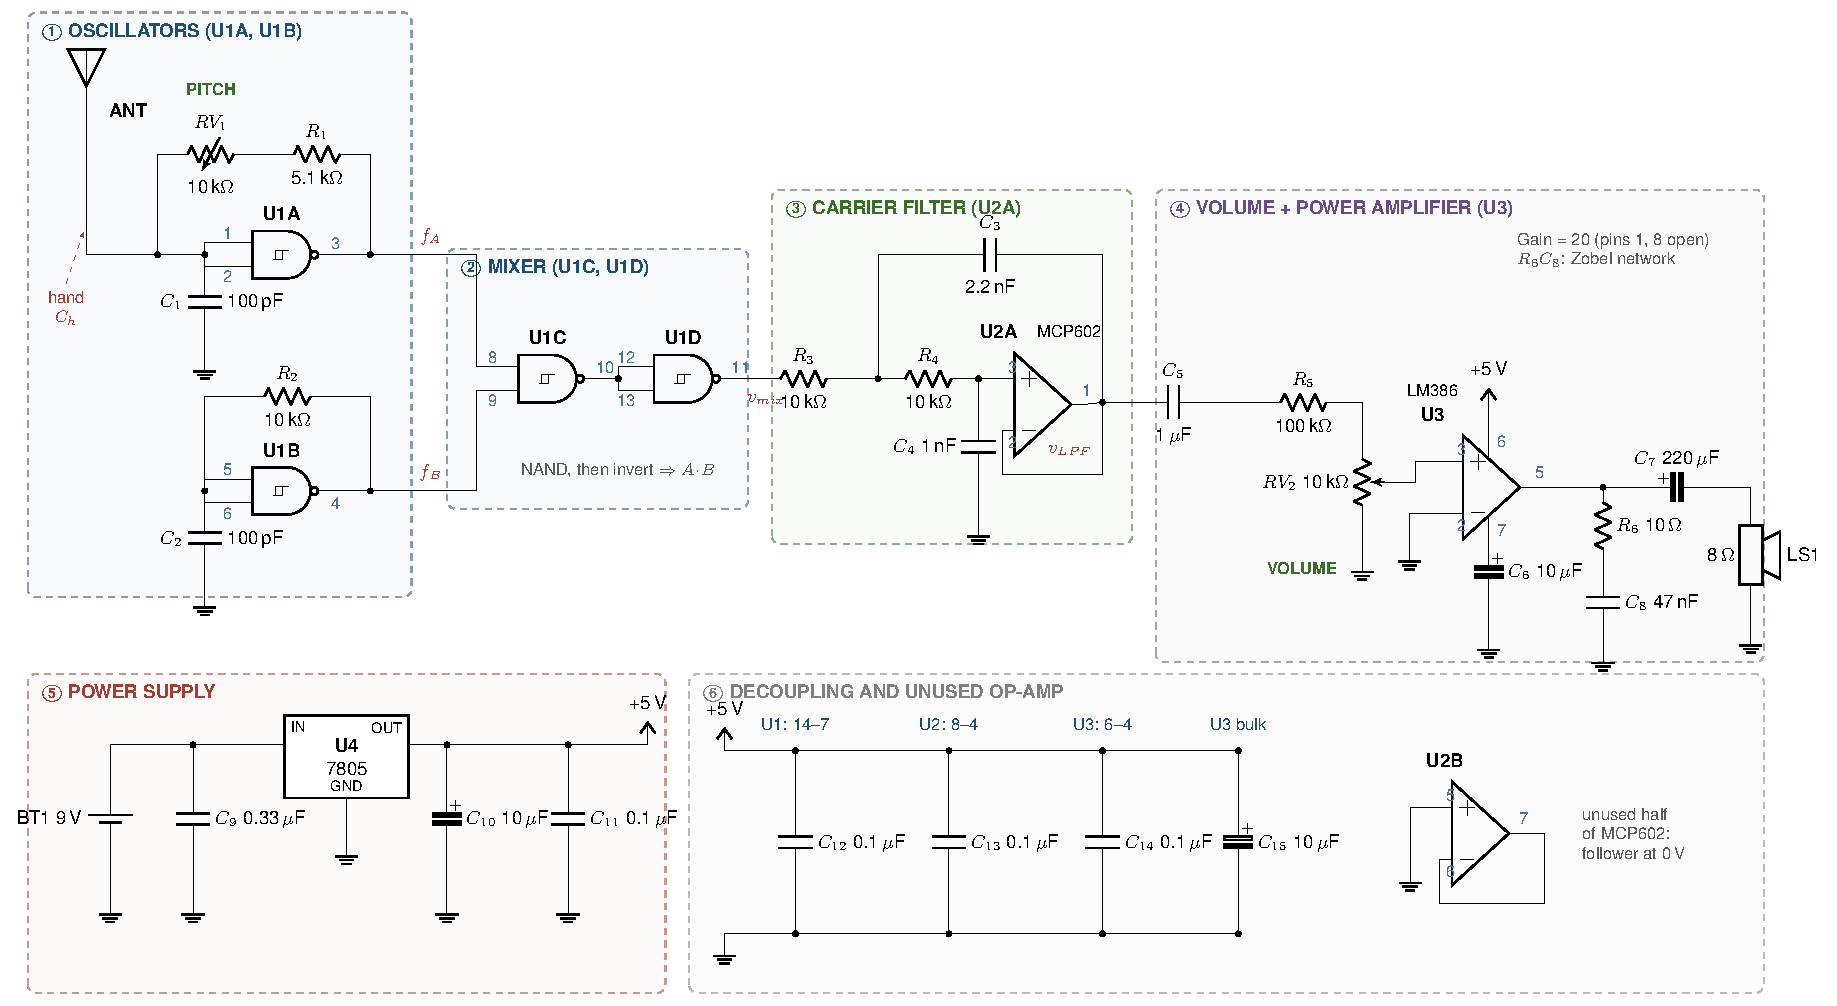
\includegraphics[width=\textwidth]{figs/schematic.pdf}
\caption{Complete schematic. \textcircled{\scriptsize 1} Antenna and reference oscillators (U1A, U1B). \textcircled{\scriptsize 2} NAND mixer and inverter (U1C, U1D). \textcircled{\scriptsize 3} Sallen--Key carrier filter (U2A). \textcircled{\scriptsize 4} Attenuator, volume control and LM386 power amplifier. \textcircled{\scriptsize 5} 9\,V battery and 7805 regulator. \textcircled{\scriptsize 6} Supply decoupling and the unused MCP602 half. Blue numbers are IC pin numbers; red italic labels mark the signals analysed in Section~\ref{sec:design}.}
\label{fig:sch}
\end{figure*}

%=====================================================================
\section{Circuit Design and Analysis}\label{sec:design}

\subsection{Schmitt-Trigger RC Oscillator}
Each oscillator is a CD4093 gate with both inputs tied together, so it acts as a Schmitt inverter. A resistor feeds back from output to input, and a capacitor runs from input to ground~\cite{horowitz2015}. The capacitor charges until it reaches the upper threshold $V_P$ and then discharges until it reaches the lower threshold $V_N$. A simple analysis ignores the gate propagation delay $t_{pd}$. During that delay, however, the capacitor keeps moving, so each half-cycle actually starts beyond the threshold, at
\begin{equation}
V_H=V_{DD}-(V_{DD}-V_P)\,e^{-t_{pd}/\tau},\qquad V_L=V_N\,e^{-t_{pd}/\tau},
\label{eq:overshoot}
\end{equation}
where $\tau=(R+r_o)C$ and $r_o$ is the gate's output resistance. The period is then
\begin{equation}
T=\tau\left[\ln\frac{V_{DD}-V_L}{V_{DD}-V_P}+\ln\frac{V_H}{V_N}\right]+2t_{pd}.
\label{eq:period}
\end{equation}
With CD4093 typical values at $V_{DD}=5$\,V ($V_P=2.9$\,V, $V_N=1.9$\,V, $t_{pd}=190$\,ns, $r_o\approx400\,\Omega$~\cite{cd4093}), the reference oscillator ($R_2=10$\,k$\Omega$, $C_2=100$\,pF) gives $V_H=3.26$\,V, $V_L=1.58$\,V and $T=1.445\,\mu$s, so \textbf{$f_B=692$\,kHz} with a duty cycle of $D=48.2\%$.

\novel{The $1/(1.2RC)$ rule of thumb is 20\% high.} The widely quoted estimate gives 833\,kHz here. It ignores both the delay and the overshoot it causes, and at this frequency they add $\approx$0.5\,$\mu$s to a 1.4\,$\mu$s period. Because the CD4093 is operating near its speed limit, delay makes up a large, device-dependent share of $T$. This is why the two oscillators must be matched on the same die (Section~\ref{sec:disc}).

\subsection{Antenna Sensitivity}
The antenna connects directly to the timing node of U1A. Its self-capacitance, $C_{ant}\approx8$\,pF (an estimate for a short wire and lead), and the hand capacitance $C_h$ both add to $C_1$. Evaluating (\ref{eq:period}) numerically at the zero-beat operating point gives
\begin{equation}
\left|\frac{\partial f_A}{\partial C}\right| \approx 3.9\ \text{kHz/pF},
\label{eq:sens}
\end{equation}
so a change of 0.26\,pF moves the pitch by 1\,kHz. The naive estimate $f\,\Delta C/C$ used in many hobby write-ups, evaluated with the 833\,kHz rule, gives 8.3\,kHz/pF, which overstates the sensitivity by more than a factor of two.

\subsection{Hybrid Potentiometer--Antenna Pitch Control}
U1A's feedback path is $R_1=5.1$\,k$\Omega$ in series with the 10\,k$\Omega$ pitch pot $RV_1$. With the hand absent, zero beat ($f_A=f_B$) occurs at $RV_1=4.13$\,k$\Omega$, slightly below mid-travel. Over its full travel the pot sweeps $f_A$ from 0.94 to 0.51\,MHz (Fig.~\ref{fig:pitch}b), which easily absorbs component tolerances and the unknown antenna capacitance. That is its first role.

Its second role is musical. Adding $C_h$ always \emph{lowers} $f_A$. If the pot is set so that $f_A<f_B$ with no hand present, an approaching hand widens the gap and the pitch rises \emph{monotonically}. Turning the pot a little further sets a chosen base note, which the hand then bends upward (Fig.~\ref{fig:pitch}a). This offset also keeps the two oscillators away from exact zero beat. Near zero beat, two weakly coupled oscillators on a shared supply tend to \emph{injection-lock}~\cite{adler1946}, which creates the silent ``dead zone'' familiar to theremin builders.

The pot's tuning slope is $|\partial f_A/\partial RV_1|=43.5$\,Hz/$\Omega$. On a 270$^\circ$ single-turn 10\,k$\Omega$ pot, that is $\approx$1.6\,kHz per degree, so the pot acts as a coarse control that the hand then refines.

\begin{figure*}[!t]
\centering
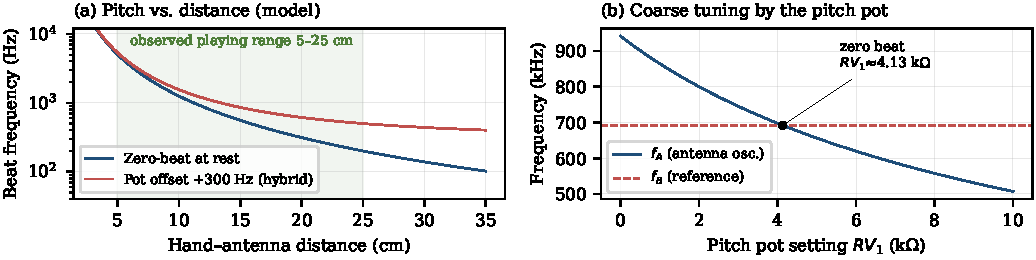
\includegraphics[width=0.92\textwidth]{figs/pitch.pdf}
\caption{(a) Beat frequency versus hand distance, from (\ref{eq:sens}) and an illustrative hand-capacitance model $C_h(d)=1.29\,\text{pF}\,(5\,\text{cm}/d)^2$ calibrated to the observed 5--25\,cm playing range. The hybrid pot offset raises the lowest note to a chosen base pitch. (b) Antenna-oscillator frequency versus pitch-pot setting from (\ref{eq:period}); zero beat occurs at $RV_1=4.13$\,k$\Omega$.}
\label{fig:pitch}
\end{figure*}

\subsection{Logic-Gate Mixer}
U1C forms $\overline{A\cdot B}$ and U1D inverts it, giving $A\cdot B$. Let $\theta(t)$ be the phase offset between the two square waves, measured as a fraction of one carrier period and wrapped to $(-\tfrac12,\tfrac12]$. This offset advances steadily at the beat rate, $\theta=f_b t$. For a duty cycle $D\le\tfrac12$, both inputs are high for a fraction $\max(0,D-|\theta|)$ of each carrier period. Averaged over the carrier, the mixer output is therefore
\begin{equation}
\bar v_{mix}(t)=V_{DD}\,\max\!\big(0,\;D-|\theta(t)|\big),
\label{eq:tri}
\end{equation}
which is a \novel{triangle wave at $f_b$} running from $0$ to $V_{DD}D=2.41$\,V. A triangle wave contains only odd harmonics, with amplitudes $\propto1/n^2$: the third is $-19.1$\,dB and the fifth $-28$\,dB relative to the fundamental, for a total harmonic distortion of 12\%. This produces the soft, flute-like timbre of the instrument, and the timbre comes from the mixer itself rather than from a separate waveshaper.

\novel{Why the inverter U1D is needed.} The raw NAND output of U1C would average between $V_{DD}(1-D)=2.59$\,V and $5$\,V. That exceeds the MCP602's input common-mode limit of $V_{DD}-1.2=3.8$\,V~\cite{mcp602}, so the waveform would be clipped. Inverting it moves the signal down to 0--2.41\,V, safely inside the valid range. The otherwise spare fourth gate therefore works as an exact level shifter at no extra cost.

\subsection{Carrier Filter (U2A)}
The unity-gain Sallen--Key filter uses $R_3=R_4=10$\,k$\Omega$, $C_3=2.2$\,nF (feedback) and $C_4=1$\,nF (to ground), which gives
\begin{equation}
f_c=\frac{1}{2\pi R\sqrt{C_3C_4}}=10.7\ \text{kHz},\qquad Q=\frac{1}{2}\sqrt{\frac{C_3}{C_4}}=0.74 .
\label{eq:sk}
\end{equation}
The response is flat over the 0.1--5\,kHz playing band and attenuates the 692\,kHz carrier by 72\,dB in the ideal model (Fig.~\ref{fig:bode}). At the carrier, the op-amp's finite output impedance sets a real stopband floor. However, the LM386's bandwidth and the loudspeaker suppress any residue further.

\begin{figure}[!t]
\centering
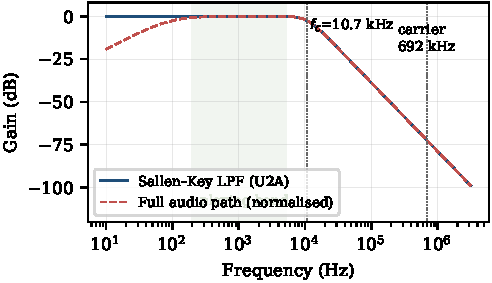
\includegraphics[width=\columnwidth]{figs/bode.pdf}
\caption{Frequency response of the Sallen--Key filter alone and of the full audio path including the $C_5$ and $C_7$ coupling networks (normalised). The shaded band is the playing range.}
\label{fig:bode}
\end{figure}

\subsection{Output Stage}
$C_5$ (1\,$\mu$F) blocks the 1.2\,V DC level of the triangle. Its time constant with the 108\,k$\Omega$ load is 0.11\,s, so the output settles quickly at switch-on, and the high-pass corner of 1.5\,Hz leaves the audio untouched. $R_5=100$\,k$\Omega$ and the 10\,k$\Omega$ volume pot $RV_2$, in parallel with the LM386's 50\,k$\Omega$ input, form a 1:13 attenuator. At full volume the amplifier input is therefore 0.19\,V\,p-p, and at the LM386's default gain of 20 (pins 1 and 8 open~\cite{lm386}) this reaches the $\approx$3.6\,V\,p-p output limit at 5\,V. The volume pot can thus use its full travel without heavily overdriving the amplifier. $C_7=220\,\mu$F couples the 8\,$\Omega$ speaker with a 90\,Hz high-pass corner. The Zobel network $R_6C_8$ and the pin-7 bypass $C_6$ follow the datasheet recommendations~\cite{lm386}.

\subsection{Power Supply}
A 7805~\cite{lm7805} regulates the 9\,V battery to 5\,V for all three ICs, with $C_9=0.33\,\mu$F at its input as the datasheet recommends. A regulated rail keeps the CD4093 thresholds and delays, and therefore $f_A$ and $f_B$, independent of battery discharge. Each IC has a 0.1\,$\mu$F decoupling capacitor, and the LM386 has an extra 10\,$\mu$F bulk capacitor. Table~\ref{tab:power} gives the estimated budget. Consumption is about 11\,mA at idle and roughly 50\,mA during typical playing, which gives an estimated 6--10\,h from a 9\,V alkaline cell. Regulation holds until the battery falls to about 7\,V (the 7805's 2\,V dropout).

\begin{table}[!t]
\centering
\caption{Estimated power budget (5\,V rail, 9\,V battery)}
\label{tab:power}
\footnotesize
\setlength{\tabcolsep}{4pt}
\begin{tabular}{@{}lrl@{}}
\toprule
Block & Current & Basis \\
\midrule
CD4093BE, 4 gates at $\approx$0.7\,MHz & $\approx$1.5\,mA & estimate ($CV^2f$ + RC) \\
MCP602, both halves & 0.46\,mA & 230\,$\mu$A/amp typ.~\cite{mcp602} \\
LM386 quiescent & 4\,mA & typ.~\cite{lm386} \\
7805 quiescent & $\approx$5\,mA & typ.~\cite{lm7805} \\
\midrule
\textbf{Idle total} & \textbf{$\approx$11\,mA} & $\approx$0.1\,W from 9\,V \\
Speaker at moderate volume & $\approx$40\,mA & estimate \\
\textbf{Typical playing} & \textbf{$\approx$50\,mA} & 7805 dissipates $\approx$0.2\,W \\
\bottomrule
\end{tabular}
\end{table}

%=====================================================================
\section{Implementation}\label{sec:impl}
The prototype was built on a solderless breadboard (Fig.~\ref{fig:proto}). A twisted copper-wire lead serves as the pitch antenna, and there is a panel potentiometer for pitch and a second for volume. Table~\ref{tab:bom} lists the parts. The two 100\,pF timing capacitors should be matched C0G/NP0 ceramics, so that zero beat falls inside the pot's range and stays put as temperature changes.

\begin{figure}[!t]
\centering
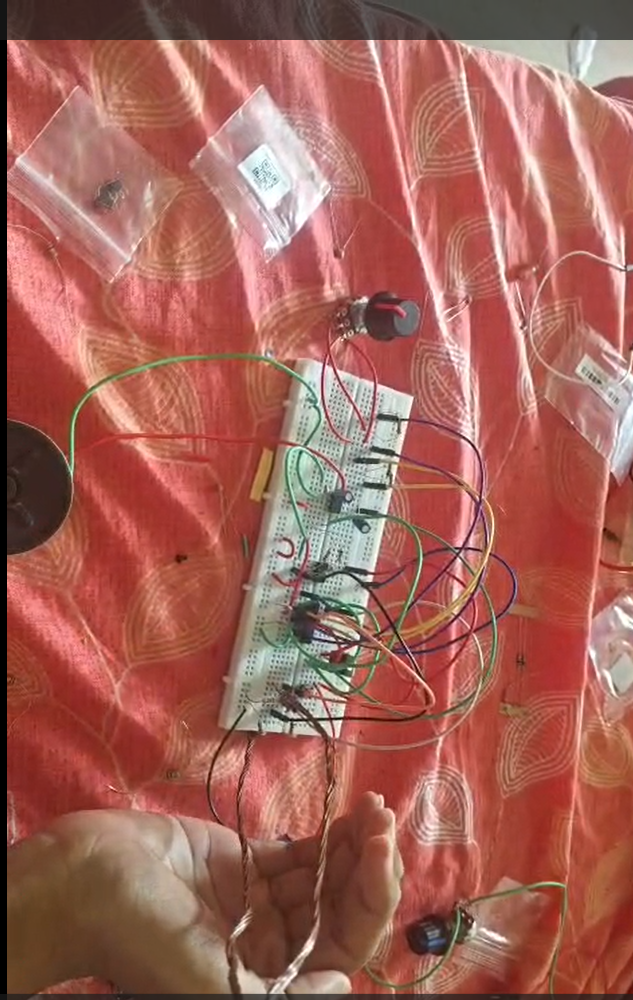
\includegraphics[angle=90,width=\columnwidth]{figs/prototype.png}
\caption{Breadboard prototype being played. The twisted-wire antenna (right, beside the hand), pitch potentiometer, the three ICs and the 8\,$\Omega$ speaker (bottom) are visible.}
\label{fig:proto}
\end{figure}

\begin{table}[!t]
\centering
\caption{Bill of materials}
\label{tab:bom}
\footnotesize
\setlength{\tabcolsep}{3pt}
\begin{tabular}{@{}llp{3.7cm}@{}}
\toprule
Ref. & Value / part & Function \\
\midrule
U1 & CD4093BE & Oscillators, mixer, inverter \\
U2 & MCP602 & Sallen--Key filter; U2B unused \\
U3 & LM386 & Speaker amplifier, gain 20 \\
U4 & 7805 & 5\,V regulator \\
$R_1$, $RV_1$ & 5.1\,k$\Omega$, 10\,k$\Omega$ pot & Antenna-osc.\ timing; pitch \\
$R_2$ & 10\,k$\Omega$ & Reference-osc.\ timing \\
$C_1$, $C_2$ & 100\,pF C0G & Oscillator timing (matched) \\
$R_3$, $R_4$ & 10\,k$\Omega$ & Sallen--Key resistors \\
$C_3$, $C_4$ & 2.2\,nF, 1\,nF & Sallen--Key capacitors \\
$C_5$ & 1\,$\mu$F film & DC block \\
$R_5$, $RV_2$ & 100\,k$\Omega$, 10\,k$\Omega$ pot & Attenuator; volume \\
$C_6$, $C_7$ & 10\,$\mu$F, 220\,$\mu$F elec. & LM386 bypass; speaker coupling \\
$R_6$, $C_8$ & 10\,$\Omega$, 47\,nF & Zobel network \\
$C_9$ & 0.33\,$\mu$F & Regulator input \\
$C_{10}$, $C_{15}$ & 10\,$\mu$F elec. & Regulator output; U3 bulk \\
$C_{11}$--$C_{14}$ & 0.1\,$\mu$F & Rail and IC decoupling \\
ANT, LS1, BT1 & wire, 8\,$\Omega$, 9\,V & Antenna, speaker, battery \\
\bottomrule
\end{tabular}
\end{table}

\textbf{Tuning procedure.} (1) Switch on with hands at least 50\,cm from the antenna. (2) Turn $RV_1$ slowly until the tone sweeps down through zero beat, which is heard as a low growl that falls silent. (3) Continue a few degrees in the direction in which an approaching hand makes the pitch \emph{rise}, and stop at the desired base note. (4) Set the level with $RV_2$.

%=====================================================================
\section{Results}\label{sec:results}
\subsection{Full-Circuit SPICE Verification}
Because no bench instruments were available during the build, the complete netlist of Fig.~\ref{fig:sch} was simulated in ngspice. The model uses behavioural CD4093 gates with datasheet thresholds, a 190\,ns delay and 400\,$\Omega$ outputs, an MCP602 macromodel (2.8\,MHz GBW, rail-to-rail output) and an LM386 model (gain 20, 50\,k$\Omega$ inputs). Table~\ref{tab:verify} compares the hand analysis with the simulation, and they agree to within 0.05\% on every oscillator value. With $RV_1$ set 23\,$\Omega$ above zero beat, which by the 43.5\,Hz/$\Omega$ slope should give 1.00\,kHz, the simulated beat is exactly 1.00\,kHz. Fig.~\ref{fig:wave} shows the waveforms: the carriers, the AND-gate output, the recovered triangle, and the speaker voltage.

\begin{table}[!t]
\centering
\caption{Hand analysis versus full-circuit SPICE simulation}
\label{tab:verify}
\footnotesize
\setlength{\tabcolsep}{3pt}
\begin{tabular}{@{}lrr@{}}
\toprule
Quantity & Analysis & SPICE \\
\midrule
Reference frequency $f_B$ & 692.1\,kHz & 692.2\,kHz \\
$f_A$ at $RV_1=0$ & 941.6\,kHz & 941.3\,kHz \\
$f_A$ at $RV_1=2$\,k$\Omega$ & 800.1\,kHz & 799.8\,kHz \\
$f_A$ at $RV_1=4.16$\,k$\Omega$ & 690.8\,kHz & 690.6\,kHz \\
Beat at $RV_1=4.153$\,k$\Omega$ & 1.00\,kHz & 1.00\,kHz \\
U2A output range & 0--2.41\,V & 0.02--2.39\,V \\
U2A output mean & 1.20\,V & 1.16\,V \\
Speaker, full volume & $\le$3.6\,V\,p-p & 2.7\,V\,p-p \\
\bottomrule
\end{tabular}
\end{table}

\begin{figure}[!t]
\centering
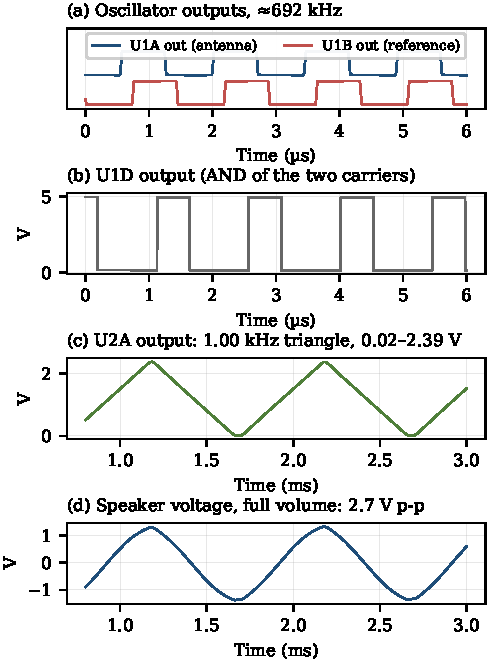
\includegraphics[width=\columnwidth]{figs/waveforms.pdf}
\caption{Full-circuit SPICE waveforms. (a) Oscillator outputs. (b) AND-gate (U1D) output, whose pulse width tracks the phase difference. (c) U2A output: a 1.00\,kHz triangle, as predicted by (\ref{eq:tri}). (d) Speaker voltage at full volume, slightly rounded as the LM386 approaches its output limit.}
\label{fig:wave}
\end{figure}

The spectrum in Fig.~\ref{fig:spec} confirms the triangle-wave prediction: the third harmonic is 19.2\,dB below the fundamental, matching the $1/n^2$ law, and the carrier is suppressed by about 70\,dB.

\begin{figure}[!t]
\centering
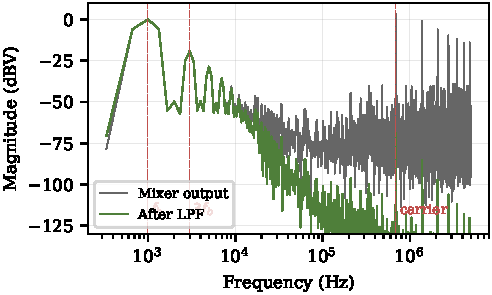
\includegraphics[width=\columnwidth]{figs/spectrum.pdf}
\caption{Spectra of the mixer output and the filtered output. The beat fundamental and its odd harmonics pass, and the carrier cluster near 692\,kHz is removed.}
\label{fig:spec}
\end{figure}

\subsection{Experimental Observations}
Powered from a 9\,V battery, the breadboard prototype behaved as the analysis predicts:
\begin{itemize}
\item A steady tone was heard at power-up, confirming that both oscillators were running with the beat in the audible range.
\item Moving a hand toward the antenna raised the pitch, and moving it away lowered the pitch. The change was smooth and continuous, with no audible steps, over roughly 5--25\,cm from the antenna.
\item The pitch pot set the base note, and changing the volume did not shift the pitch.
\item AC coupling at the speaker removed the DC offset and clearly improved sound quality compared with a direct connection.
\item Long battery leads caused slight pitch drift, and nearby metal objects shifted the base pitch. Both effects follow from (\ref{eq:sens}), as discussed below.
\end{itemize}
Fig.~\ref{fig:pitch}(a) shows the pitch--distance relation implied by (\ref{eq:sens}). Because the hand-capacitance law depends on geometry, that curve is a calibrated model, not a measurement.

%=====================================================================
\section{Discussion}\label{sec:disc}
\textbf{Common-mode drift cancellation.} By (\ref{eq:period}), each frequency depends on $V_P$, $V_N$, $t_{pd}$ and $r_o$, and all of these vary with temperature and from device to device. The CD4093 datasheet allows $V_P$ anywhere from 2.2 to 3.6\,V at 5\,V~\cite{cd4093}. On two separate chips, this spread could shift the two frequencies by tens of percent relative to each other, which no pot could null. On one die the variations are common-mode, and because only $f_A-f_B$ is heard, first-order drift cancels.

\textbf{Environmental sensitivity.} At 3.9\,kHz/pF, a stray change of only 0.03\,pF, such as a lead moving a few millimetres, shifts the pitch by about 100\,Hz. This explains the observed sensitivity to battery-lead length and to nearby metal. Short, fixed wiring and a grounded enclosure are the practical remedies.

\textbf{Limitations.} (i) Tuning with a single-turn pot is coarse, at about 1.6\,kHz per degree. (ii) The hybrid offset reduces injection locking near zero beat but does not eliminate it. (iii) The linear regulator wastes about 44\% of the battery power. (iv) There is no volume antenna, so loudness is set by hand. (v) The quantitative results come from simulation, and bench measurements remain to be done.

%=====================================================================
\section{Conclusion and Future Work}
We have presented a three-IC, inductor-free heterodyne theremin in which one CD4093BE performs every RF function. Closed-form models explain its operating frequency, antenna sensitivity, playing range and triangle-wave timbre, and a full-circuit SPICE simulation confirms the oscillator values to within 0.05\%. The analysis also shows two design constraints that are easy to miss: the inverter stage is needed to respect the op-amp's input range, and the oscillators must be matched on a single die. The hybrid pot--antenna control and the single 9\,V supply make the instrument practical and portable. Future work includes bench measurements with an oscilloscope and spectrum analyser, a multi-turn or varactor fine-tuning control, a second antenna for volume, a low-dropout regulator, and a PCB with a guarded antenna trace.

\section*{Acknowledgment}
The authors thank Dr.~Jitendra Goyal for his guidance and support. This work was carried out as part of the analog electronics curriculum at Vellore Institute of Technology, Vellore.

\begin{thebibliography}{99}
\footnotesize
\raggedright
\bibitem{theremin1928} L.~S.~Theremin, ``Method of and apparatus for the generation of sounds,'' U.S. Patent 1\,661\,058, Feb. 28, 1928.
\bibitem{skeldon1998} K.~D.~Skeldon, L.~M.~Reid, V.~McInally, B.~Dougan, and C.~Fulton, ``Physics of the Theremin,'' \emph{Amer. J. Phys.}, vol.~66, no.~11, pp.~945--955, Nov. 1998.
\bibitem{moog1961} R.~A.~Moog, ``A transistorized theremin,'' \emph{Electronics World}, Jan. 1961.
\bibitem{glinsky2000} A.~Glinsky, \emph{Theremin: Ether Music and Espionage}. Urbana, IL, USA: Univ. of Illinois Press, 2000.
\bibitem{greatscott} GreatScottLab, ``Make your own simple theremin,'' Instructables. [Online]. Available: \url{https://www.instructables.com/Make-Your-Own-Simple-Theremin/}
\bibitem{sallenkey1955} R.~P.~Sallen and E.~L.~Key, ``A practical method of designing RC active filters,'' \emph{IRE Trans. Circuit Theory}, vol.~CT-2, no.~1, pp.~74--85, Mar. 1955.
\bibitem{franco2015} S.~Franco, \emph{Design With Operational Amplifiers and Analog Integrated Circuits}, 4th~ed. New York, NY, USA: McGraw-Hill, 2015.
\bibitem{horowitz2015} P.~Horowitz and W.~Hill, \emph{The Art of Electronics}, 3rd~ed. Cambridge, U.K.: Cambridge Univ. Press, 2015.
\bibitem{cd4093} Texas Instruments, ``CD4093B types: CMOS quad 2-input NAND Schmitt triggers,'' datasheet. [Online]. Available: \url{https://www.ti.com/lit/ds/symlink/cd4093b.pdf}
\bibitem{adler1946} R.~Adler, ``A study of locking phenomena in oscillators,'' \emph{Proc. IRE}, vol.~34, no.~6, pp.~351--357, Jun. 1946.
\bibitem{mcp602} Microchip Technology, ``MCP601/1R/2/3/4: 2.7\,V to 6.0\,V single supply CMOS op amps,'' datasheet DS21314. [Online]. Available: \url{https://www.microchip.com/en-us/product/MCP602}
\bibitem{lm386} Texas Instruments, ``LM386 low voltage audio power amplifier,'' datasheet. [Online]. Available: \url{https://www.ti.com/lit/ds/symlink/lm386.pdf}
\bibitem{lm7805} Texas Instruments, ``LM340, LM340A and LM7805 family wide VIN 1.5-A fixed voltage regulators,'' datasheet. [Online]. Available: \url{https://www.ti.com/lit/ds/symlink/lm7800.pdf}
\end{thebibliography}

\end{document}
